\chapter{Event Simulation}
\label{sim}
%somewhere have the pretty picture from 
%matt mc tutorial on how generators/geant/etc 
%fit in with everything else (reco, whatever)

%ARXIV PAPER OF AWESOMENESS
%http://arxiv.org/abs/hep-ph/0403045

%PYTHIA MANUAL OF AWESOMENESS
% the one I'm looking at is lutp0613man2.pdf, 
% but there's probably a more recent one




% I THINK I HAVE TOO MANY LONG SENTENCES 
% AND PREPOSITIONAL PHRASES


%need for event simulation: 

Within %the role of % CHANGE THIS CONSTRUCTION
a high-energy physics experiment's role of making 
discoveries and measurements, 
it necessary to know ahead of time what exactly 
should be expected. 
What will the detector signature of a new process look like? 
How will we know whether we've seen something unexpected? 
This is where event simulation contributes.  
%what exactly is the simulated data
Essentially, a series of programs is used to carefully 
generate and calculate all the relevant quantities for a set of 
fake events.  
This information is then used 
to aid analysis in ways for which 
real data alone cannot suffice.  

Having the ability to simulate physics processes 
serves multiple purposes. 
It aids in detector design: 
knowing the expected typical characteristics of particle 
interactions is essential to design a detector 
suited for those interactions.  
Once the detector design is settled, 
simulation of the detector is useful to design 
the algorithms used to reconstruct particles 
from their signature interactions with the 
detector material.  
In addition, simulating the physics processes 
can give estimates of how many 
events of a particular type are expected, 
further aiding the design process.  
The event simulation also contributes 
directly to many analyses, 
in the way of calculating the acceptance, 
the fraction of events that can theoretically 
be detected (see Section~\ref{FIXME}): 
it is impossible to know from observation 
how many events are missed by the detector, 
because of the very fact that they are unseen.  
It is instead necessary to get that fraction 
from a framework in which 
the characteristics of all events are 
inherently known, not reconstructed.  
Finally, % and possibly most visibly (?) I don't like that
simulated data is directly compared 
with ``real'' data from the detector 
to interpret the real-data results.  
If the data shows something significantly 
different from the simulation, 
then something is missing: 
perhaps a calibration needs to be applied, 
or the response of a detector unit needs 
to be further understood.  
Or, perhaps, there is a new physics process 
appearing for the first time, 
which was not previously known and 
which was therefore not present in the simulation.  
In this case simulation of proposed new physics 
processes may narrow down the identity of the 
observed new process.  
Whatever the case, 
discrepancy between observed data and the event 
simulation indicates that further 
investigation is necessary.  


%points of event simulation: 

%   * directly relevant: compare with data (description of current understanding as is) 
%-- we want to be able to interpret what we're seeing 
%in terms of what physics process it might be

%   * also relevant: acceptance is necessarily a MC calculation!

%   * also: design detectors, design reconstruction and other (e.g. trigger) algorithms

%   * also: event rates (like trigger rates?)  

The entire detection process is simulated, 
including the protons' direct interaction 
and any subsequent particle decays, 
as well as how the end-product particles 
interact with the detector as they pass through 
and how the detector itself responds.  
This latter part includes not only the 
material of the individual subdetectors 
but also the algorithms of 
the Level-1 Trigger, 
which are implemented in hardware 
(see Section~\ref{exp:L1}).  
The High-Level Trigger does not need to be 
simulated in this way; 
since its algorithms are all software-based, 
the same code can be run without modification 
on both real data and simulated data.  



\section{Monte Carlo Event Generation}
\label{sim:MC}

``Event generation'' refers to 
creating a set of fake physics events, 
usually realistic, 
for purposes of study and 
comparison with real data.  
The term ``Monte Carlo'' is connected 
with this process 
because at the most basic level 
it is based on random numbers.  
All physics interactions happen in 
terms of probabilities: 
process X is more likely to happen than 
process Y, 
so process X is observed more often.  
For any given fake event, 
which physics process is actually simulated 
is randomly determined 
according to those probabilities.  
The kinematics of the event 
(energies and directions of incoming 
and outgoing particles) 
are also assigned according to 
probabilities.  
The final result is that having enough events 
will reproduce the original probabilities 
of each interaction.  
(It is worth noting that in terms of software, 
nothing is really random; in general, 
programs to create ``random numbers''
are really only pseudorandom.  
However, for the purpose of event generation, 
pseudorandom numbers are suitable if 
they are sufficiently random-like.  
Moreover, using a deterministic 
pseudorandom generation algorithm 
aids in debugging -- 
the results of the algorithm are reproducible, 
which cannot happen with truly random numbers.)  

%put why called ``monte carlo'', 
%also connect ``event simulation'' terminology 
%with ``generator'' and the multiple types thereof.
%like, ``simulation'' broken down into several steps, 
%one of which is the generation of the main 
%physics process itself (aka ``hard physics process'')
%HOW the events are actually ``generated'', 
%like the whole random number business. 
%It uses a random number generator , 
%to determine ``in a probabilistic way'' -- 
%only one main interaction happens 
%for each proton (bunch) interaction, 
%but the sum over all events ,
%according to the probability of each type of 
%interaction happening.  



\subsection{Types of Monte Carlo Simulation Programs}
\label{sim:MCexplain}

%types of programs with different types of output -- what they're used for. 
%start with tree-level stuff and dsigma eqn...

%   * cross section integrators

%   * event generators

There are two sorts of programs that can be called 
%``Monte Carlo generators''.  
``Monte Carlo event simulators''.  
They both use the matrix elements derived from 
the Feynman diagrams of the physics interactions of interest 
(explained in Section~\ref{FIXME}), % THAT MEANS EXPLAIN ALL THIS STUFF IN PREVIOUS CHAPTER
but they use the matrix element formalism 
in different ways to achieve different ends.  
As a reminder, the equation to obtain the 
differential cross section % WHAT'S IT ACTUALLY CALLED??
from the matrix element for a given diagram is 

\[
d\sigma = \frac{1}{\hat{s}}|\mathcal{M}|^2 \frac{d \cos \theta d\phi}{8(2\pi)^2}
\]

The first type of Monte Carlo program outputs 
a single quantity or set of quantities characteristic 
of the given process, 
such as the cross section.  
These programs are called ``cross section integrators''.  
They calculate 
$d\sigma$ for each of a uniform distribution of 
phase space vales (i.e. uniform increments 
of $\cos\theta$ and $\phi$).  
$d\sigma$ represents each event's ``weight''; 
the total cross section $\sigma$ is then obtained 
by integrating over the full collection of $d\sigma$ values.  
The final result is a value for the cross section; 
hence the name.  
However, since the events themselves are distributed 
uniformly in $\cos\theta$ and $\phi$, 
their characteristics 
do not represent actual event distributions 
(real event distributions in data have 
non-uniform distributions, 
in $\cos\theta$ in particular).  
Therefore they can only be used to calculate 
a few select quantities; 
they can't be used to predict distributions.  

The second type of program are called ``event generators''.  
They also use the matrix element to calculate 
the differential cross section element % REAL NAME ?
with the equation given above.  
However, instead of using $d\sigma$ as an event weight, 
it ``unweights'' the events to obtain the physical 
distributions.  
It does this through the so-called acceptance-rejection method: 
first the maximum possible value of $d\sigma$ is calculated, 
$d\sigma_{max}$. 
Each event's individual $d\sigma$ value, 
the ratio $\frac{d\sigma}{d\sigma_{max}}$ is taken; 
this number is necessarily a fraction between 0 and 1.  
A random number $g$ between 0 and 1 is then generated.  
If the ratio $\frac{d\sigma}{d\sigma_{max}}$ is greater 
than $g$, then then event is kept.  
Otherwise, it is rejected.  
This method causes the generated events to have the properties 
and distributions that events would have in reality -- 
sections of phase space with a higher ``event weight'' 
are more likely to be represented.  

%tree-level all well and good, but need corrections to really 
%make things realistic.  
%ways of doing the corrections:

%   * matrix element

%   * parton shower

However, using a single Feynman diagram is not typically 
sufficient to make very accurate calculations.  
%a number or determine distributions is not typically 
%sufficient.  
In general, there are significant contributions from 
the higher-order diagrams  
(diagrams with more legs and loops, 
but still representing the same final arrangement of particles). 
These corrections must be taken into account.  
In addition, the matrix elements and Feynman diagrams 
for these calculations only consider bare quarks, 
that is, quarks extracted from the framework of 
hadrons such as the proton.  
These bare quarks cannot exist in reality, 
so a method of accounting for the quarks 
as being inside hadrons must also be used.  
There have been two different paths taken to deal % path = tack? track?...
with the above issues.  
In the first, the ``matrix element'' method, 
Higher-order diagrams are explicity included in 
the matrix element calculation.  
Since the higher the order, 
the more complex the calculation, 
only diagrams of up to a given order are 
generally used.  
In one implementation, more ``legs'' can be dealt with, 
but diagrams containing virtual loops are ignored.  % EXPLAIN IN PREVIOUS CH
In the other, all diagrams, including those with virtual 
loops, of a single order are used, 
but at the moment there exist satisfactory solutions 
only for next-to-leading-order diagrams 
(or NLO, explained in Section~\ref{FIXME}).  
%only for diagrams one step higher 
%than the basic tree-level diagram
The matrix element method does not explicitly 
take care of the bare-quark problem; %, though.  
this can be handled in multiple ways.  
%Programs who do not deal with the interactions of 
Some cross section integrators deal with the interactions of % is it only cross section integrators??
quarks inside hadrons using Feyman's factorization theorem. 
Programs which do not deal with them in this way 
can be interfaced with programs following the 
second of the two paths, %.  
%The second path is called 
the ``parton shower'' method, 
which is the method used by many event generators 
(as opposed to cross section integrators).  
In the parton shower method, 
instead of including diagrams representing 
higher orders and quarks-within-hadrons 
into the matrix element calculation, 
this part of the interaction is taken care of 
by a separate routine.  
This routine takes the products of the 
basic tree-level interaction 
and decays them according to 
probabilities and rules coded into the program.  
The process is iterative, 
repeating for any quarks or gluons that 
branch off at any point.  
In this way the parton shower method 
is more flexible than the matrix element method -- 
it can deal with many branchings and legs. 
However, it is also less precise formally, 
since it avoids the use of the matrix elements 
from the Feynman diagrams.  

%where do the PDFs fit in?  just to parton shower method?? 
%no, it looks like PDFs have to enter in both 
%ways of doing hadronization. 
%(actually, is it only just the initial 
%proton interaction where you need the PDFs?? 
%inside a proton is the only place 
%where x is a relevant quantity...
%dunno, skirt for now)

%do I need more detail at this point?  
%I guess still need to explain modular structure... 
%can more specific stuff like hadronization 
%model go just under pythia, or should it 
%go here?  
%I guess should be more general, 
%since those algorithms are more general.  
%SO, HERE

The philosophy of parton-shower generators 
in particular 
is that the entire process of simulating 
a physics event can be done in a modular fashion.  
Fig.~\ref{fig:MCsteps} 
shows the typical steps necessary to simulate an events.  
The incoming protons are modeled in terms of the 
parton distribution functions (Section~\ref{FIXME}).  % NEED TO EXPLAIN ``PARTONS'' IN THAT SECTION
The ``hard subprocess'' refers to the main 
physics interaction.  
Not shown in the diagram are other interactions 
involving different parts of the protons 
or other protons in the same bunch; 
these interactions, known as the ``underlying event,''  
are often not as interesting physics-wise 
because they are typically not as energetic.  
The participant particles in the main interaction 
are then ``evolved'' through the showering process, 
which includes emissions of photons or gluons 
by the initial or final particles, 
as well as ``branchings'' of final particles. % INCLUDED IN FORMER?? 
Any resulting quarks and gluons are 
formed into ``colorless'' hadrons, % but gluons colorless to being with -- and do they ``form'' into hadrsons??
% no, I think gluons are NOT colorless -- you wouldn't be able to get ggg vertices
which may then decay into other particles. 
These final particles are the ones seen 
in the detector.  
The fact that the full process can be separated 
into these steps 
makes it easier for different programs 
to handle individual steps.  
For example, one program may simulate the 
hard process, 
while another is better-equipped to take care 
of the showering and hadronization, 
and a third is specialized in the decay of 
a particular particle.  
To further the theme of modularity, 
the fully-decayed situation 
is then plugged into a program simulating 
the passage of the particles through the detector 
and the detector's response (Section~\ref{FIXME}).  

%need to explain since not actually using jets 
%in analysis, but there may be jets in final state
%%(and need to define ``jet'' -- FIXME MORE FOR THEORY SECTION)
%from ISR and FSR
The process of hadronization is not directly 
relevant to this analysis, 
since it does not require hadrons to 
exist in the final state.  
However, since initial- or final-state radiation 
may cause jets incidental to the main interaction 
that nevertheless affect its kinematics, 
hadronization is dealt with here.  
%CAN TREAT ELECTRONS ETC AS ``PARTONS'' AND 
%INCLUDE QED IN SHOWERING -- makes framework easier 
%(maybe put in pythia section?  
%can't remember if it's pythia-specific)
In addition, it simplifies things to treat 
electrons and photons in the final state as ``partons'', 
in the same category as the quarks and gluons.  
Even though they are not constituents of the proton, 
they can be modeled as having 
``distribution functions'' 
and subject to ``showers'' of 
photons and electrons. 
Therefore different sorts of processes can be 
plugged into the same machinery and treated the same way.  

%all this stuff on QCD isn't directly relevant for my 
%stuff, should maybe concentrate more on mine... 
%show the feynman diagram again?  

%parton-shower is default pythia method (for QCD), 
%but matrix element can be used

%And how these two things fulfill the different needs for 
%both higher orders and hadronization

%BIG PRETTY PARTON SHOWER PICTURE but also need to explain PDF part, etc. etc. 
%should compare to other one from zeus people, which one is better? 

 \begin{figure}[htb]
  \begin{center}
    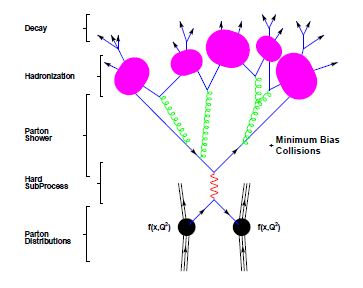
\includegraphics{Figures/mc-partonShower-lesHouches.png}
  \end{center}
  \caption[Diagram of typical steps used to simulate event in parton shower method]
	  {Diagram of typical steps used to simulate event in parton shower method.
	    The incoming protons are modeled in terms of the 
	    parton distribution functions. 
	    The ``hard subprocess'' refers to the main 
	    physics interaction.  
	    The participant particles in the main interaction 
	    are then ``evolved'' through the showering process, 
	    which includes emissions of photons or gluons 
	    by the initial or final particles, 
	    as well as ``branchings'' of final particles. % INCLUDED IN FORMER?? 
	    Any resulting quarks and gluons are 
	    formed into ``colorless'' hadrons, 
	    which may then decay into other particles. 
	    These final particles are the ones seen 
	    in the detector.  
	  }
  \label{fig:MCsteps}
 \end{figure}


%\subsection{some explanation of the black box?}
%\label{sim:MCBlackBox}
% it's not really a black box anymore!
%can talk about black-box mentality in introduction
%modular structure here?  that pretty picture showing all the 
%different steps to an interaction that need to be 
%simulated. 
%all those steps can be done by separate packages, 
%which is the philosophy.  (pythia manual)
%pdfs ->
%hard scatter (underlying event, multiple interactions in parallel) ->
%[parton] shower (both isr and fsr, incl QED) ->
%hadronization (not directly applicable to my process, but applicable for bg's) -> 
%decay resonances -> interactions with detector material ...

\subsection{Monte Carlo Generator Programs}
\label{sim:MCGens}

%short intro on programs: pythia, powheg, tauola, fewz

%HOW THE PROGRAMS USED TO GENERATE THESE SAMPLES AND NUMBERS 
%FIT INTO THIS FRAMEWORK.  

Several Monte Carlo programs were used to fulfill 
different roles in this analysis.  
Two programs were used to generate the simulation events used: 
one general-purpose generator for background events, 
and a more specialized generator for the signal sample.  
A few of the background samples used a dedicated decay 
program to decay specific particles in the end state.  
Finally, a cross section integrator was used to 
obtain a highly precise estimate of the theoretical 
value of the interaction cross section.  
These programs will be detailed in the following sections.  


%   pythia, powheg, tauola, fewz... else??  (didn't end up using MCatNLO) 
%I don't think anything else.  
%also explain about fewz different (xsec integrator, sounds like)

%I feel like I remember seeing something from herwig?? in one of the 
%production config fragments...

\subsubsection{PYTHIA}
\label{sim:MCGensPythia}

%PYTHIA THE MONSTER

%   * general-purpose parton-shower event generator

%   * pdfs, main process, showering, hadronization, decays

%   * implements many beyond-standard model processes for study

%   * lots of stuff built up over the years, but doesn't do everything


CMS makes use of one of the standard 
Monte Carlo event generation workhorses, 
a program known as PYTHIA.  
PYTHIA is a general-purpose event generator 
using the parton-shower approach to corrections.  
It encompasses most of the steps necessary to generate 
an event: 
the parton distribution functions 
that describe the colliding protons, 
the main physics interaction process, 
and how the end products shower, 
hadronize, and decay.  
Over its long history PYTHIA has built up 
a large collection of tools, 
which include many main physics processes and 
various methods of dealing with each of the steps 
mentioned above.  
PYTHIA also includes many non-standard-model 
physics processes 
in order to study new physics theories.  
Most of what it does can be adjusted by the user 
via changing parameters; 
however, its default values are chosen to produce 
valid output without the need to 
necessarily adjust settings.  
Because PYTHIA is such a wide-ranging program, 
it does not treat everything it handles in depth.  
For this reason, specialized programs are sometime used 
to work with specific areas of the simulation process, 
including the ones in the following sections.  


%and lund string model pictures (both, yay!)
This analysis does not directly deal with 
quarks or jets; 
however, since jets can be present in the final state 
and can play a role in the kinematics of the \Zee 
interaction, 
the method of dealing with jets and the QCD 
processes that form them is relevant here.  
PYTHIA by default uses the Lund string model 
(shown schematically in Fig.~\ref{fig:MClund})
to evolve 
quarks and gluons through the process of hadronization 
and formation into jets. %, 
Conceptually, an interaction's final state may have 
quarks 
%and/or gluons 
``flying off in different directions''.  
However, quarks cannot exist alone: %.  % and gluons?
they must always exist with other quarks, 
held together by the strong force.  
If the individual quarks do not have very much energy 
as they move apart, 
the increasing energy of their interaction will hold them together.  
However, if the quarks have much energy, 
the interaction energy will not be enough to hold 
them together, 
and they will need to form new ``quark partners'' 
in order to not be alone.  
According to the Lund string model, 
%linear confinement -- 
the energy between opposite color charges 
increases approximately linearly with distance. 
The energy is concentrated into a linear area, 
like a tube or string.  
These strings are always stretched between two quarks.  
Enough energy on the part of the quarks will 
``break'' the string and 
create a new quark-antiquark pair, 
which then fills the need for ``quark partners'', 
as illustrated in Fig~\ref{fig:MClundB}.  
The process continues until quarks 
do not have enough energy to overcome 
the force holding them together.  % wishy-washy use of ``force''?

 \begin{figure}[htb]
  \begin{center}
%    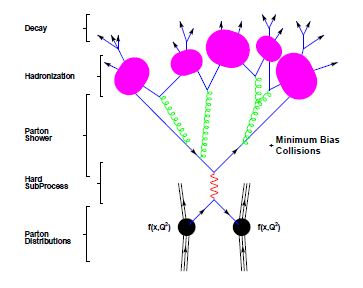
\includegraphics{Figures/mc-partonShower-lesHouches.png}
    \subfloat[]{\label{fig:MClundA}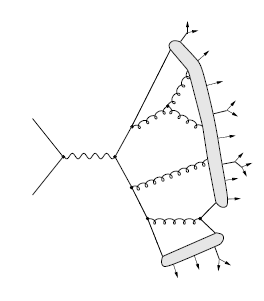
\includegraphics{Figures/mc-lundStringDiagram-zeusPeople.png}}
    \subfloat[]{\label{fig:MClundB}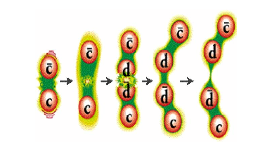
\includegraphics{Figures/mc-lundStringModel-zeusPeople.png}}
  \end{center}
  \caption[Schematics showing the Lund string model of hadronization]
	  {Schematics showing the Lund string model of hadronization.
	  \subref{fig:MClundA} In the Lund string model, the quarks 
	  are joined by strings which ``break'' to form new 
	  quark-antiquark pairs. 
	  The process continues until the quarks' energies are  
	  not enough to overcome the force holding them together.  
	  The gray areas represent chains of quarks joined by such strings.  
	  \subref{fig:MClundB} An illustration of a possible 
	  creation of a quark-antiquark pair.  
	  }
  \label{fig:MClund}
 \end{figure}

%pythia is definitely parton shower, 
%explain steps and hadronization model, etc


%what are the different tunes for?  tune z2, tune d6t 
%actually, I think they're for the underlying event

%https://twiki.cern.ch/twiki/bin/view/CMS/PythiaTuning

%so NOT just CMS-based, they're pythia-wide.  
%but I don't see Z2 or D6T on this page: 
%http://home.fnal.gov/~skands/leshouches-plots/

The underlying event 
can be represented in PYTHIA 
by different configurations of parameters, 
known as ``tunes.''  
The tunes have been chosen to correctly model 
already-existing distributions from previous 
experiments.  
This analysis uses samples generated 
according to the default tune used in CMS, 
Tune Z2.  
However, differences between the tunes 
are very slight and affect 
final results very little; 
these affects are accounted for 
in the systematic errors 
(Section~\ref{anMeth:SystsOther}).  

\subsubsection{POWHEG}
\label{sim:MCGensPowheg}
%why is this one used for signal in favor of pythia?  
%more to the point, what exactly is it? 
%and how is it different from pythia? 

%http://www-zeuthen.desy.de/~alioli/talks/Granada.pdf  POWHEG 
%explanatory talk of AWESOMENESS

POWHEG (for ``POsitive Weight Hardest Emission Generator'') 
is a method for making next-to-leading order (NLO) 
corrections within a parton shower framework.  
At low energies, the showering algorithms implemented 
in parton shower generators 
model the corrections well.  
However, at higher energies, a next-to-leading order 
matrix calculation is more accurate.  
An ideal solution combines the two approaches 
to get the best of each.  
Since POWHEG does this, 
it therefore produces a more accurate picture 
of the radiation corrections and their effects 
on final-state kinematic quantities 
when compared to a standard parton-shower 
generator such as PYTHIA, 
which only include some (the real part) 
of these corrections.  
POWHEG consists of a number of routines representing 
various main physics processes, 
including \Zee.  
Processes that are not already included 
in the set may be implemented by the user.  

POWHEG was used to generate the 
hard process for each event 
of the \Zee signal sample; 
this part of the interaction was then 
fed through PYTHIA 
(by the modular procedure previously described) 
to undergo hadronization.  
It was more important for the signal 
sample to be accurate to higher order 
than for the background samples; 
the background samples are only of interest 
in terms of how much they may contaminate 
the signal sample.  
Slight variations in their distributions 
due to missing higher-order corrections are 
therefore not relevant.  

% don't really need anything else?  
% not from experimentalist point of view!(?)
% experimentalist don't talk about 
% angular-ordered showers


\subsubsection{Other Generators}
\label{sim:MCGensOther}
%Like, whichever other samples I check (background etc) -- actually, they're all pythia

%or just have separate sections for both as for pythia and powheg?  

%TAUOLA AND FEWZ

Two other Monte Carlo event generators 
played roles in the analysis.  
In the first case, 
particles in some of the background samples 
called for a specialized decay package.  
In the second, 
a precise theoretical prediction was needed 
to compare with data, 
and the standard programs used to generate 
the events 
cannot reach the necessary precision.  

%\subsubsubsection{TAUOLA}
%\label{sim:MCGensTauola}

%the first reference for TAUOLA is always
%S. Jadach, J. H. Kuhn, and Z. Was, Comput.
%Phys. Commun. 64 (1990) 275.
% not mentioned in VBTF

% but other refs through the years: 
%http://arxiv.org/abs/hep-ph/0411377
%http://arxiv.org/abs/hep-ph/0610386
%http://arxiv.org/abs/1101.1652

%homepage given as http://wasm.home.cern.ch/wasm/goodies.html
%REAL homepage for any useful stuff is the f77: http://wasm.home.cern.ch/wasm/f77.html
%(c++ page only has interface-specific stuff)

% also abstract included in les houches guidebook -- didn't find it anywhere else

Many particle decays are handled by 
the primary event generator, PYTHIA.  
However, there are several aspects of decays 
that PYTHIA does not deal with, 
such as spin polarization.  
Because these aspects can have small effects 
on the kinematic distributions of the decayed 
particles, 
CMS decided to use a separate package, TAUOLA, 
to decay tau particles in the samples 
that included taus.  
%While TAUOLA implements non-standard interactions, % NEED THIS?????
%this is not made use of here.  
%Only standard decays are used.  
TAUOLA specifically takes spin polarization 
into account, 
and includes first order QED corrections.  % WHY NOT [need] QCD?? can decay hadronically!
The TAUOLA package was only necessary for the 
Z->tau tau and W->tau nu background samples.  % PRETTIFY

%\subsubsubsection{FEWZ}
%\label{sim:MCGensFewz}

%AND, FEWZ webpage was on frank petriello's wisconsin space and doesn't exist anymore

%http://www.phys.hawaii.edu/~kirill/FEHiP.htm links to 
%http://www.hep.wisc.edu/~frankjp/FEWZ.html (bad link)

%FEWZ 2.0 abstract on the arXiv: http://arxiv.org/abs/1011.3540 
%from ryan gavin, ye li, frank petriello, and seth quackenbush (15 Nov 2010)

%WHICH VERSION DID VBTF USE??  look at syst AN.  
%e-mail frank about documentation page??

%HA HERE'S THE NEW PAGE: http://gate.hep.anl.gov/fpetriello/FEWZ.html

%https://indico.cern.ch/getFile.py/access?contribId=38\&resId=3\&materialId=slides\&confId=71330  
%tutorial from ryan giving original arXiv references (non-2.0)

%   * arxiv:hep-ph/0603182, arxiv:hep-ph/0609070 -- okay, both of those are calculation papers, not necessarily software papers

%okay, the second one actually mentions fewz. 
%(and the first is only W, so just need second, I think)
%AND, vbtf gives no other references than those two.  
%So I guess that's all there is!

The theoretical prediction for the cross section value 
was obtained with FEWZ, 
a cross section integration program 
specifially dealing with production of the W and Z.  
Previously, all calculations of the cross section 
had been done at next-to-leading order (NLO) in QCD, 
which entails several percent uncertainty.  
However, since the statistical error on 
W and Z results at the LHC 
was quickly expected to reach the order of 1\%, 
it was deemed necessary to undertake 
a calculation at next-to-next-to-leading order (NNLO), 
which gives a theoretical uncertainty of 
approximately the same value.  
(In essence, all higher-order corrections beyond NNLO 
contribute about a percent or less of uncertainty.)  
FEWZ was chosen to calculate the cross sections 
for the CMS analysis 
because of this treatment of NNLO QCD corrections.  


\section{Detector Simulation}
\label{sim:Detector}
%\subsection{GEANT Detector Model/Modeling of Particle Interactions in Detector Material}

After the generation of the main physics process, 
and the parton showering and hadronization and decays, 
the role of the detector itself must be taken into account.  
The final, end-state, decayed particles interact with 
the detector, which causes signals representing 
the particle's position and energy to be registered.  
These must be properly modeled to know, for example, 
%the magnitude of the energy that should be associated 
%with a given signal.  
what sort of signal would result from the passage of a particle 
with a given momentum.  
In addition, the detector itself is not completely passive, 
in that it can change the properties of the 
particles passing through it during the course of measurement.  
Both of these roles necessitate a detailed simulation 
of the detector and its response.  

%ALSO NEED SOMETHING FOR ELECTRONICS, TRIGGER, ETC

\subsection{GEANT Detector Model}
\label{sim:DetectorGeant}

%ha ha, actually talk about geant down here, 
%modeling of matter, 
%interactions of particles with matter

%GEANT the giant

The CMS collaboration uses the software package 
GEANT4 to model the detector 
within the framework of CMSSW, 
the CMS-specific analysis software 
(see Section~\ref{FIXME}).  
GEANT4 provides a toolkit designed 
to accurately represent all facets of 
the detector simulation.  
These include the ability to construct 
a precise geometrical model of the 
detector itself, 
complete with any actual misalignments 
and a model of the detector's magnetic field, 
as well as the physical properties 
of the materials used.  
In addition, the package also handles 
the properties of the 
fundamental particles involved, 
how they behave in the modeled 
magnetic field, 
and how they interact with the different 
materials present in the detector.  
For example, the detection of particles 
in the electromagnetic calorimeter 
depends on those particles causing 
a shower of other particles upon 
interacting with the material of the 
calorimeter; 
this must be modeled.  
Finally, GEANT4 also provides 
the ability to model the response of 
the electronics used to detect the particles, 
like the response of a photomultiplier tube 
to a light signal caused by such a shower.  

\subsection{Level-1 Trigger Emulator}
\label{sim:DetectorL1Emul}
%YAY emulator

%talk about how emulator necessary for l1, but not for hlt (duh)

In addition to modeling the detector 
components that do the actual detecting, 
it is necessary to include the response of 
the trigger system (Section~\ref{exp:trigger}), %.  
%This modeling serves several purposes.  
serving multiple purposes.  
Modeling the trigger system enables 
the estimation of event rates 
for a given luminosity 
before the experiment actually runs 
with that luminosity.  
In particular, 
this permitted the estimation of rates
long before the detector was fully constructed, 
greatly aiding the experiment's 
physics planning.  
In addition, comparison of the real-time 
``online'' performance of the trigger 
with its software counterpart 
can indicate and aid in diagnosing 
problems with the online running.  

The High-Level part of the trigger system (HLT), 
consisting of algorithms implemented in software, 
is simply run ``offline'' as an element 
of the detector simulation.  
However, the Level-1 Trigger (L1), 
being implemented in electronics 
instead of software, 
must be explicitly modeled.  
The sofware package that does this 
is called the Level-1 Trigger Emulator, 
since it aims to be a bit-by-bit 
emulation of the trigger hardware 
instead of just a simulation of the 
algorithms implemented.  
The L1 Emulator is modular in the 
same sense as the hardware system; 
information is passed between 
separate packages representing the 
different subsystems of the L1.  
Each element of the hardware, 
namely each type of processing card, 
has its own software class to handle 
its own specific functions.  
The software therefore aims overall to model 
each of the trigger's processing steps 
in accurate detail.  